\section{Introduction}

Phylogenetic comparative methods have been widely used to study species relativeness problems.
Phylogenetic models aim to find parsimonious methods that can be used to link ecological phenomena with evolutionary processes by incorporating the historical relationships shared across species via phylogenetic (evolutionary) trees. 
\ml{parsimonious can be a confusing word here}
Although such models attempt to account for species correlations, they often make strong and over-simplified assumptions of the evolutionary process. 
Decades of work have created various different methods that enables researchers to incorporate phylogenetic effects in analyzing species relativeness applications.
But many challenges remain.
In particular, accounting for phylogenetic effects in high dimensional systems is always challenging, especially for models incorporating multiple forms of phylogenetic effects, and especially with large phylogenies where computation powers are limited.
\ml{Define phylogenetic effects. PE can mean a lot of different things (see Pagel's tree transformation). What we mean here is strictly phylogenetic signal-- extent to which trait/response values are statistically related to phylogeny.}
Ignoring phylogenetic effects/signals can be problematic both biologically and statistically \citep{felsenstein1985phylogenies, li2017statistical} -- in such cases, researchers often use simpler models accounting for minimal phylogenetic signals by limiting at the individuals level and neglect additional phylogenetic signals present in the system.

Incorporating phylogenetic links between species and combine evolutionary changes with statistical processes advances the development of phylogenetic comparative methods.
The most widely used statistical process in phylogenetic comparative analysis to model evolutionary process is the pure random drift process, Brownian motion \citep{felsenstein1973maximum}. 
Although the Brownian motion is an over-simplified model of evolution, many of the existing phylogenetic comparative methods are built upon.
For example, phylogenetically independent contrasts (PICs) \citep{felsenstein1985phylogenies}, phylogenetic generalized least squares (PGLS) \citep{grafen1989phylogenetic}, Pagel's $\lambda$ \citep{pagel1999inferring}, and Blomberg's $K$ \citep{blomberg2003testing} are methods developed in the last couple of decades and have provided important insights in this field. 
Nevertheless, there are also a handful of selection beyond the pure random drift (BM) process where they probe specific aspects of the evolutionary process (i.e. Ornstein-Uhlenbeck (OU) process which accounts for both selection and drift processes, Pagel's $\delta$ and $\kappa$ transformations where it explores variation of evolutionary rates and speciational changes through time respectively).

In the past few decades, there have been an accelerating increase in discovering evolutionary history of species making historical evolutionary data accessible and at higher resolutions.
Furthermore, there have been a steadily advance of methodological research (e.g. reconstruct phylogenetic tree methods, and phylogenetic comparative methods) and observational (and meta-analysis) studies on collections of species. 
Despite the widespread use of these methods and ways to account for variability across species, groups, and different studies, there have been relatively few studies accounting for phylogenetic signals. 

\ml{write a paragraph on pglmm? Flexbility paragraph and say PIC/GLS assumes the topology and branch lengths are error free, Pagel's lambda and Blomberg's K accounts for additional tip variations of the phylogeny, to account for additional variation such as measurement error and such, people turn to Bayesian mixed models \cite{de2012bayesian, hadfield2010general}}

%The most widely used statistical method to model related species data that accounts for the phylogenetic structure is the \textit{phylogenetic regression} via independent constrast \ml{cite Felsenstein 1985} and further generalizations to generalized least square regression (PGLS) and generalized linear mixed models (PGLMM) to allow for different models of trait evolution \ml{or types of response?}. 


%Despite the choice of modelling strageties, there are many limitations in the current state of art of statistical phylogenetic analysis.
%There are a handful of studies discussing the importance of incorportating phylogenetic signals but relatively few systematically look at comparative performance of comparative phylogenetic methods. 

In this paper, we propose an alternative, yet straightforward but little-used method of constructing phylogenetic correlations directly from phylogenetic tree by summing the evolutionary changes that occurred on all of the branches in the phylogeny in its past.
\ml{flexibility: multiple obs per species and multiple levels of phylogenetic signal}
We apply relatively simple phylogenetic comparative approaches to data from simulated phylogenies that incorporate various complexity of phylogenetic signals in the model and measurement errors. 
We compare model approaches and explore various complex modelling strategies in the mixed model framework and a flexible platform for researches to explore biologically interesting questions.

We also compare three different R packages: nlme:gls, pez, phylolm, and lme4.
In principle, any given valid method should converge/get the same result/conclusion.
However, even with the relatively simple models considered here, methods that are not flexible/parameter constrained can experience problems.
Furthermore, even when different methods converge to essentially the same result, they may show large differences in computational efficiency.
\ml{Not sure if we should include the line "we are not using Bayesian approaches" here but definitely in the discussions.}

\section{Materials and Methods}

The typical phylogenetic regression is of the form:
\begin{align}
y & = XB + \epsilon \\
\epsilon & \sim MVN(0,\sigma^{2}C),
\label{eq:gls}
\end{align}
where $y$ is an $n \times 1$ vector of measurable response; $X$ is an $n \times (m + 1)$ model matrix containing 1's in the first column and the $m$ independent variable (phenotypic traits or environmental variable); $B$ is an $m + 1$ coefficient vector; $\epsilon$ is the residual error and assumed to be multivariate normally distributed with a variance-covariance matrix given by $\sigma^{2}_{\epsilon}C$ in which $C$ is an $n \times n$ matrix of the phylogenetic correlation (PC).

% More recently, researchers use linear mixed model and generalized linear mixed model framework to model complex systems with phylogenetic structures.
%\ml{Why? Data type, interactions, random effects, etc... Need to really explain random effects here. Alternatively, we can drop this line and write this...}
An alternative modelling approach is to use linear mixed effects modelling framework \citep{lynch1991methods}.
The typical linear mixed model has the form:
\begin{align}
Y & \sim F(\mu) \\
g(\mu) & = XB + Zb + \epsilon_{mm} \\
\epsilon_{mm} & \sim MVN(0,\sigma^2)
\end{align}
where $Z$ is an $n \times (m+1)$ model matrix for the $(m+1)$ -- dimensional vector-valued $m$ independent variables; $\epsilon_{mm}$ is the residual error and assumed to be multivariate normally distributed with a variance-covariance matrix given by $\sigma_{2}I$.
Analogously, the phylogenetic regression given by (1) can be represented in the mixed model framework by constraining $\epsilon_{mm} = 0$ and $Z=Z^{c}$ where the PC is incorporated in the random effect matrix. 

\subsection{Phylogenetic Tree Transformation}
The standard problem of phylogenetic comparative methods is to analyze relationships among data where the observations are gathered from nodes (usually tips) of a phylogenetic tree.
Phylogenetic independent contrasts is a generalization of the paired comparisons method where contrasts are taken for each bifurcation (nodes) in a phylogenetic tree. 
Assuming that traits evolve independently in each lineage following speciation, then the trait divergences that occur at one node are independent of divergence at other nodes.  

An alternative approach is to model the phylogenetic correlation as a \textit{Gaussian process}. 
In particular, suppose that the evolutionary process is a Brownian motion, which means the evolution of a continuous trait is a random walk and daughter species after speciation are all independent.  
In that case, the phylogenetic variability of a particular observation can be written as the sum of the evolutionary changes that occurred on all of the branches in the phylogeny in its past. 
Thus, the evolutionary history for each species can be model with a sequence of independent errors, rather than having to impose a correlation structure on the random effects. 

The random-effect model matrix $Z$ can be decomposed into term-wise model matrix $Z_{i}$ as described in \ml{in text citation lme4}.
Thus, the phylogenetic correlated random-effect matrix $Z^{C}_{i}$ is

\begin{equation}
Z^{C}_{i} = (S^{T}_{i}J^{T}_{i} \ast X^{T}_{i})^{T},
\end{equation}

\ml{double check if $l and p$ are the same with lme4}

where $\ast$ is the Khatri-Rao product, $S_{i}$ is an $l_{i} \times b_{i}$ matrix of species--branch relations; $J_{i}$ the indicator matrix of grouping factors indices matrix size $n \times l_{i}$; $X_{i}$ is the raw random effects model matrix size $n \times p_{i}$.

\ml{note: $SS^T = Cov(phylo)$ under BM assumption}
%\ml{double kronecker for interactions}


\subsection{Simulation}

We generated test data based on the simple mixed model formulation \ml{ref equation (3-5)} with a single response variable $Y$ and a single predictor continuous variable $X$ from $n$ (20, 100, and 500) species, and $m$ (1 and 20) sites. 
To account for multiple levels of phylogenetic signal, we assume phylogenetic signal in the intercept $b_0$, and slope $b_1$.
We further assume that random slope and intercept are correlated. 
For models with multiple sites, we also assume for species and site interactions random effects, an equivalent version of nested random effects or phylogenetic attraction described in \cite{helmus2007separating} with the main random effects.
Table \ml{ref something} provides the statistically equivalent fitting capabilities of common/existing phylogenetic methods.

% % \begin{table}
% % \begin{center}
% 
% \begin{tabularx}{\textwidth}{|X|X|X|}
% \hline
% Type of RE	& Formula	& Platform	\\
% \hline
% 
% Single site intercept	  &	1 $\mid$ sp	& gls (if residual = 0), phyloglm, lme4 \\
% Single site intercept and uncorrelated slopes		&  1 $\mid$ sp + trait $\mid$ sp		& lme4 \\
% Single site intercept and correlated slopes 			& 1 + trait $\mid$ sp					& lme4 \\
% \hline
% Multiple site intercept 									&  1 $\mid$ sp 						& pez, lme4 \\
% Multiple site intercept and uncorrelated slopes 	&  1 $\mid$ sp + trait $\mid$ sp 		& pez, lme4 \\
% Multiple site intercept and correlated slopes 	& 	1 + trait $\mid$ sp					& lme4 \\
% \hline
% \end{tabularx}
% % \vspace{1in}
% % ditto with site interaction								& ditto above $\mid$ sp:site		& ditto above \\
% % \end{center}
% % \end{table}

\section{Results}

\begin{center}
\begin{figure}[h]
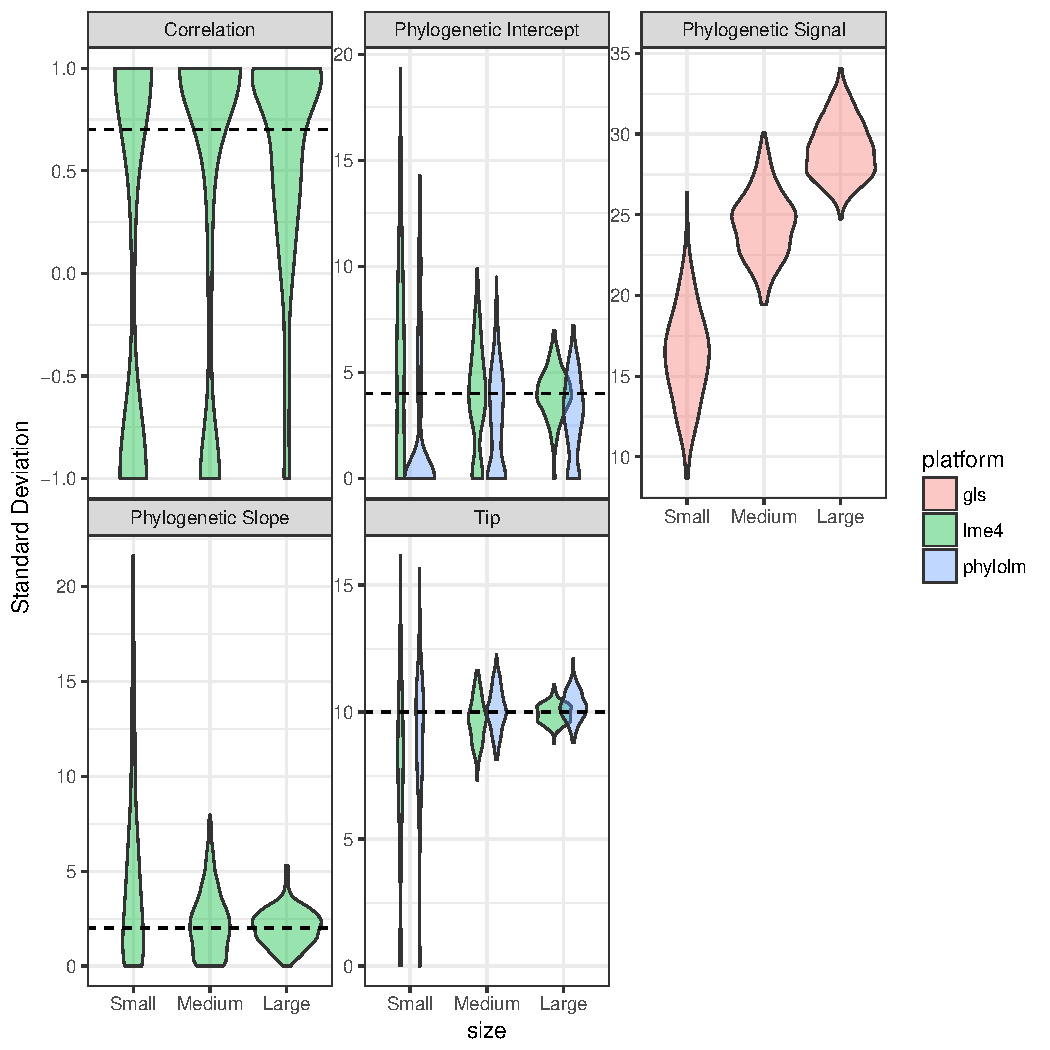
\includegraphics[scale=0.8,page=1]{./git_push/ssplot.pdf}
\label{ssplot}
\end{figure}
\end{center}

The full model (which matches the simulations model that incorporates phylogenetic signal on the intercept, slope and correlation) provides good estimates of the different levels of the phylogenetic variation signal (Figure 1 and 2).

In general, as the number of species (or phylogeny) increases, all phylogenetic signal estimates are more robust for all models (including models without random slope and correlation) except PGLS in the single site simulations. 
It is unclear how different levels of phylogenetic signal is being confounded under the error free (without tip variation) assumption for the PGLS models.
Models with only two parameters/levels of variation captures the phylogenetic intercept and tip variation reasonably well to the simulated parameters from the full model despite not including phylogenetic random slope and slope intercept correlation.

Platforms using the mixed model framework for multiple site simulations follows similar behaviour as single site simulation (i.e. as the number of species increase, different levels of phylogenetic signals and variations are closer to the simulated parameters). 
All parameter estimates are much more robust for the multiple site than the single site simulations especially slope-intercept correlations. 
There are no clear difference with phylogenetic signal models without random slope and intercept correlation.
However, despite the similarities of robustness estimation, the efficiency (measured by computational speed) of sampling independent errors in lme4 is dramatically better (orders of magnitude faster than pez.
Furthermore, it was not practical for pez to fit large sample size simulation data as the computational speed did not scale linearly.

\begin{center}
\begin{figure}[h]
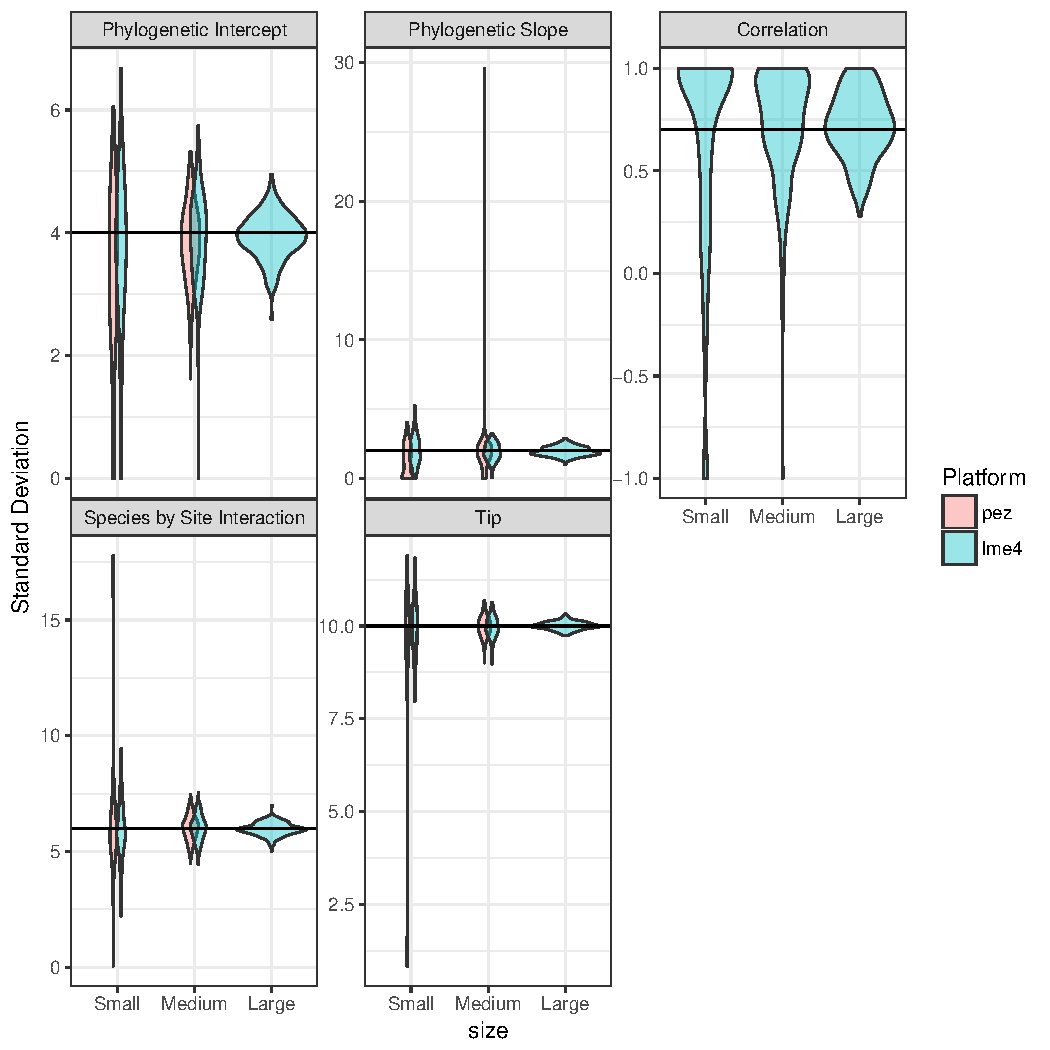
\includegraphics[scale=0.8,page=1]{./csplot.pdf}
\end{figure}
\end{center}

\begin{center}
\begin{figure}[h]
\includegraphics[scale=0.8,page=2]{./csplot.pdf}
\end{figure}
\end{center}

% \begin{center}
% \begin{figure}[h]
% 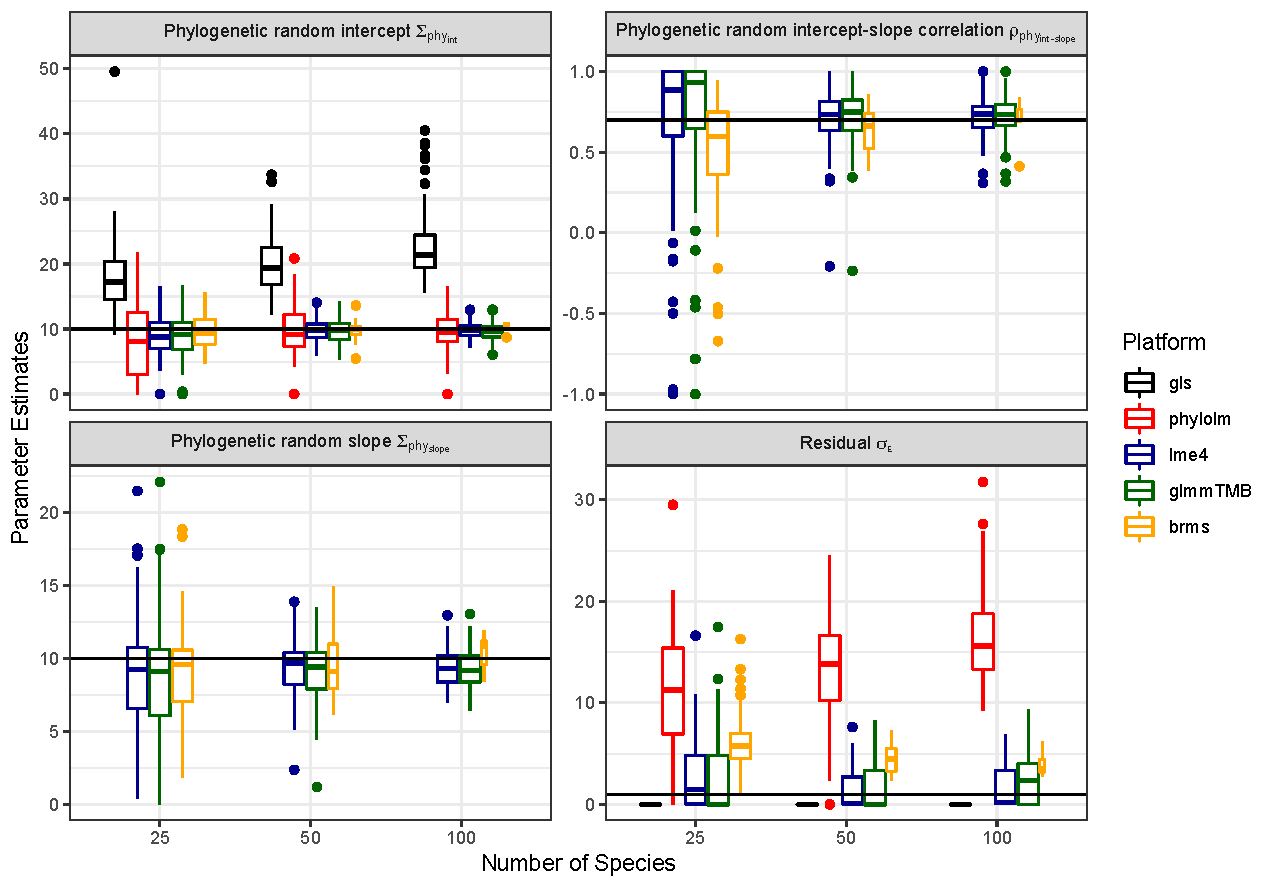
\includegraphics[scale=1]{./ssplot.pdf}
% \end{figure}
% \end{center}

\newpage

\section{Discussion}

We have fitted models including maximum capabilities to model varying levels of variation/phylogenetic signal to simulated data with ....
Using models that can include/account for multiple levels of variation is necessary for robust fits, but models that include phylogenetic signal in the intercept level can work as well as the full model.
Under the Brownian motion evolution process assumption, modelling via independent errors is much more computational efficient than imposing equivalent correlation structures.

\subsection{Process and observation errors}

Another way to think about various forms/sources of phylogenetic signals and uncertainties is characterizing into process and observation errors.
Process error or in this context, variation contributed from the evolutionary matches nicely with the variation of phylogenetic signal. 
Observation/measurement error on the other hand is harder to match in this context and data dependent.
In the classic examples, observation error is (assume to be?) zero for PIC and PGLS; single-site observation model using phylolm (or any method with two variables describing the variance (Pagel's $\lambda$, Blomberg's K)) often match the observation/measurement error with the tip variation of the phylogeny.
For multiple observations per species, the tip variation becomes one of the process errors with phylogenetic signal and the observation error is the variation among species and additional other non-process errors.

\subsection{Extension and alternatives}

Our analysis covers the classical phylogenetic comparative methods (i.e. phylogenetic least squares, linear and mixed models).
Even within the scope there is additional room for exploration we neglected, such as exploring phylogenetic multivariate response models, and phylogenetic meta analysis.
More broadly, the simple independence error approach we developed here offers a more efficient equivalent way to do Brownian motion evolution phylogenetic comparative analysis. 
This approach can in principle be combined flexibly with the state of the art phylogenetic mixed models using Bayesian frameworks such as MCMCglmm. 
More importantly, this implementation in lme4 allows users to fit phylogenetic mixed models to the fullest that other frequentest platforms? cannot (i.e. large data, unbalance species observations, complex random effects) and explore new ideas.

\section{Conclusion}

We have presented a simple approach to fit phylogenetic mixed models that is both more efficient and statistically equivalent approach and comparison of classical pcm to simulated data. 
First, this new approach is magnitudes faster compared to existing phylogenetic mixed models without losing robustness/accuracy and can easily combined with any statistically mixed model framework. 
Last and most importantly, it is more flexible in fitting large phylogenies, unbalanced datasets, and complex random effects such as slope correlations.



\newpage

\section{Supplements -- translation}

$1 \mid Sp_{phylo}$, $0 + X_{E} \mid Sp_{phylo}$ and $X_{E} \mid Sp_{phylo}$ means phylogenetically related have similar response,   

\begin{tabularx}{\textwidth}{|l|X|X|}
\hline
Formula & Statistics & Biology \\
\hline
$1 \mid Sp$ &
random species intercept; variation within species in mean response across all factors &
variation of how species respond \\
\hline

$0 + X_{E} \mid Sp$ &
random slope of environment factor within species; variation in coefficient within species for the environmental factor &
variation of how species respond to the same environmental factor \\
\hline

$1 + X_{E} \mid Sp$ &
random slope of environmental factor within species with correlated intercept; variation in coefficient within species for the environmental factor with correlated mean response across all other factors &
variation of how species respond in the same environmental factors and the correlation of the variation of how they respond in general \\
\hline

$1 \mid Site:Sp $ &
random variation in intercept among species within sites &
variation of how species respond within sites \\
\hline

$1 | Sp_{Phylo} $ &
variation among species in mean response across all factors demonstrate phylogenetic signal &
phylogenetically related species respond similarly \\
\hline

$0 + X_{E} \mid Sp_{Phylo}$ &
variation among species for environmental factors demonstrate phylogenetic signal &
phylogenetically related species respond similar (share common response) to the same environmental factor \\
\hline
\end{tabularx}
            
                                                                        
